\appendix
\chapter{Anhang}
\label{anhang}
\TODO{Formatierung}
\begin{figure}[h]
    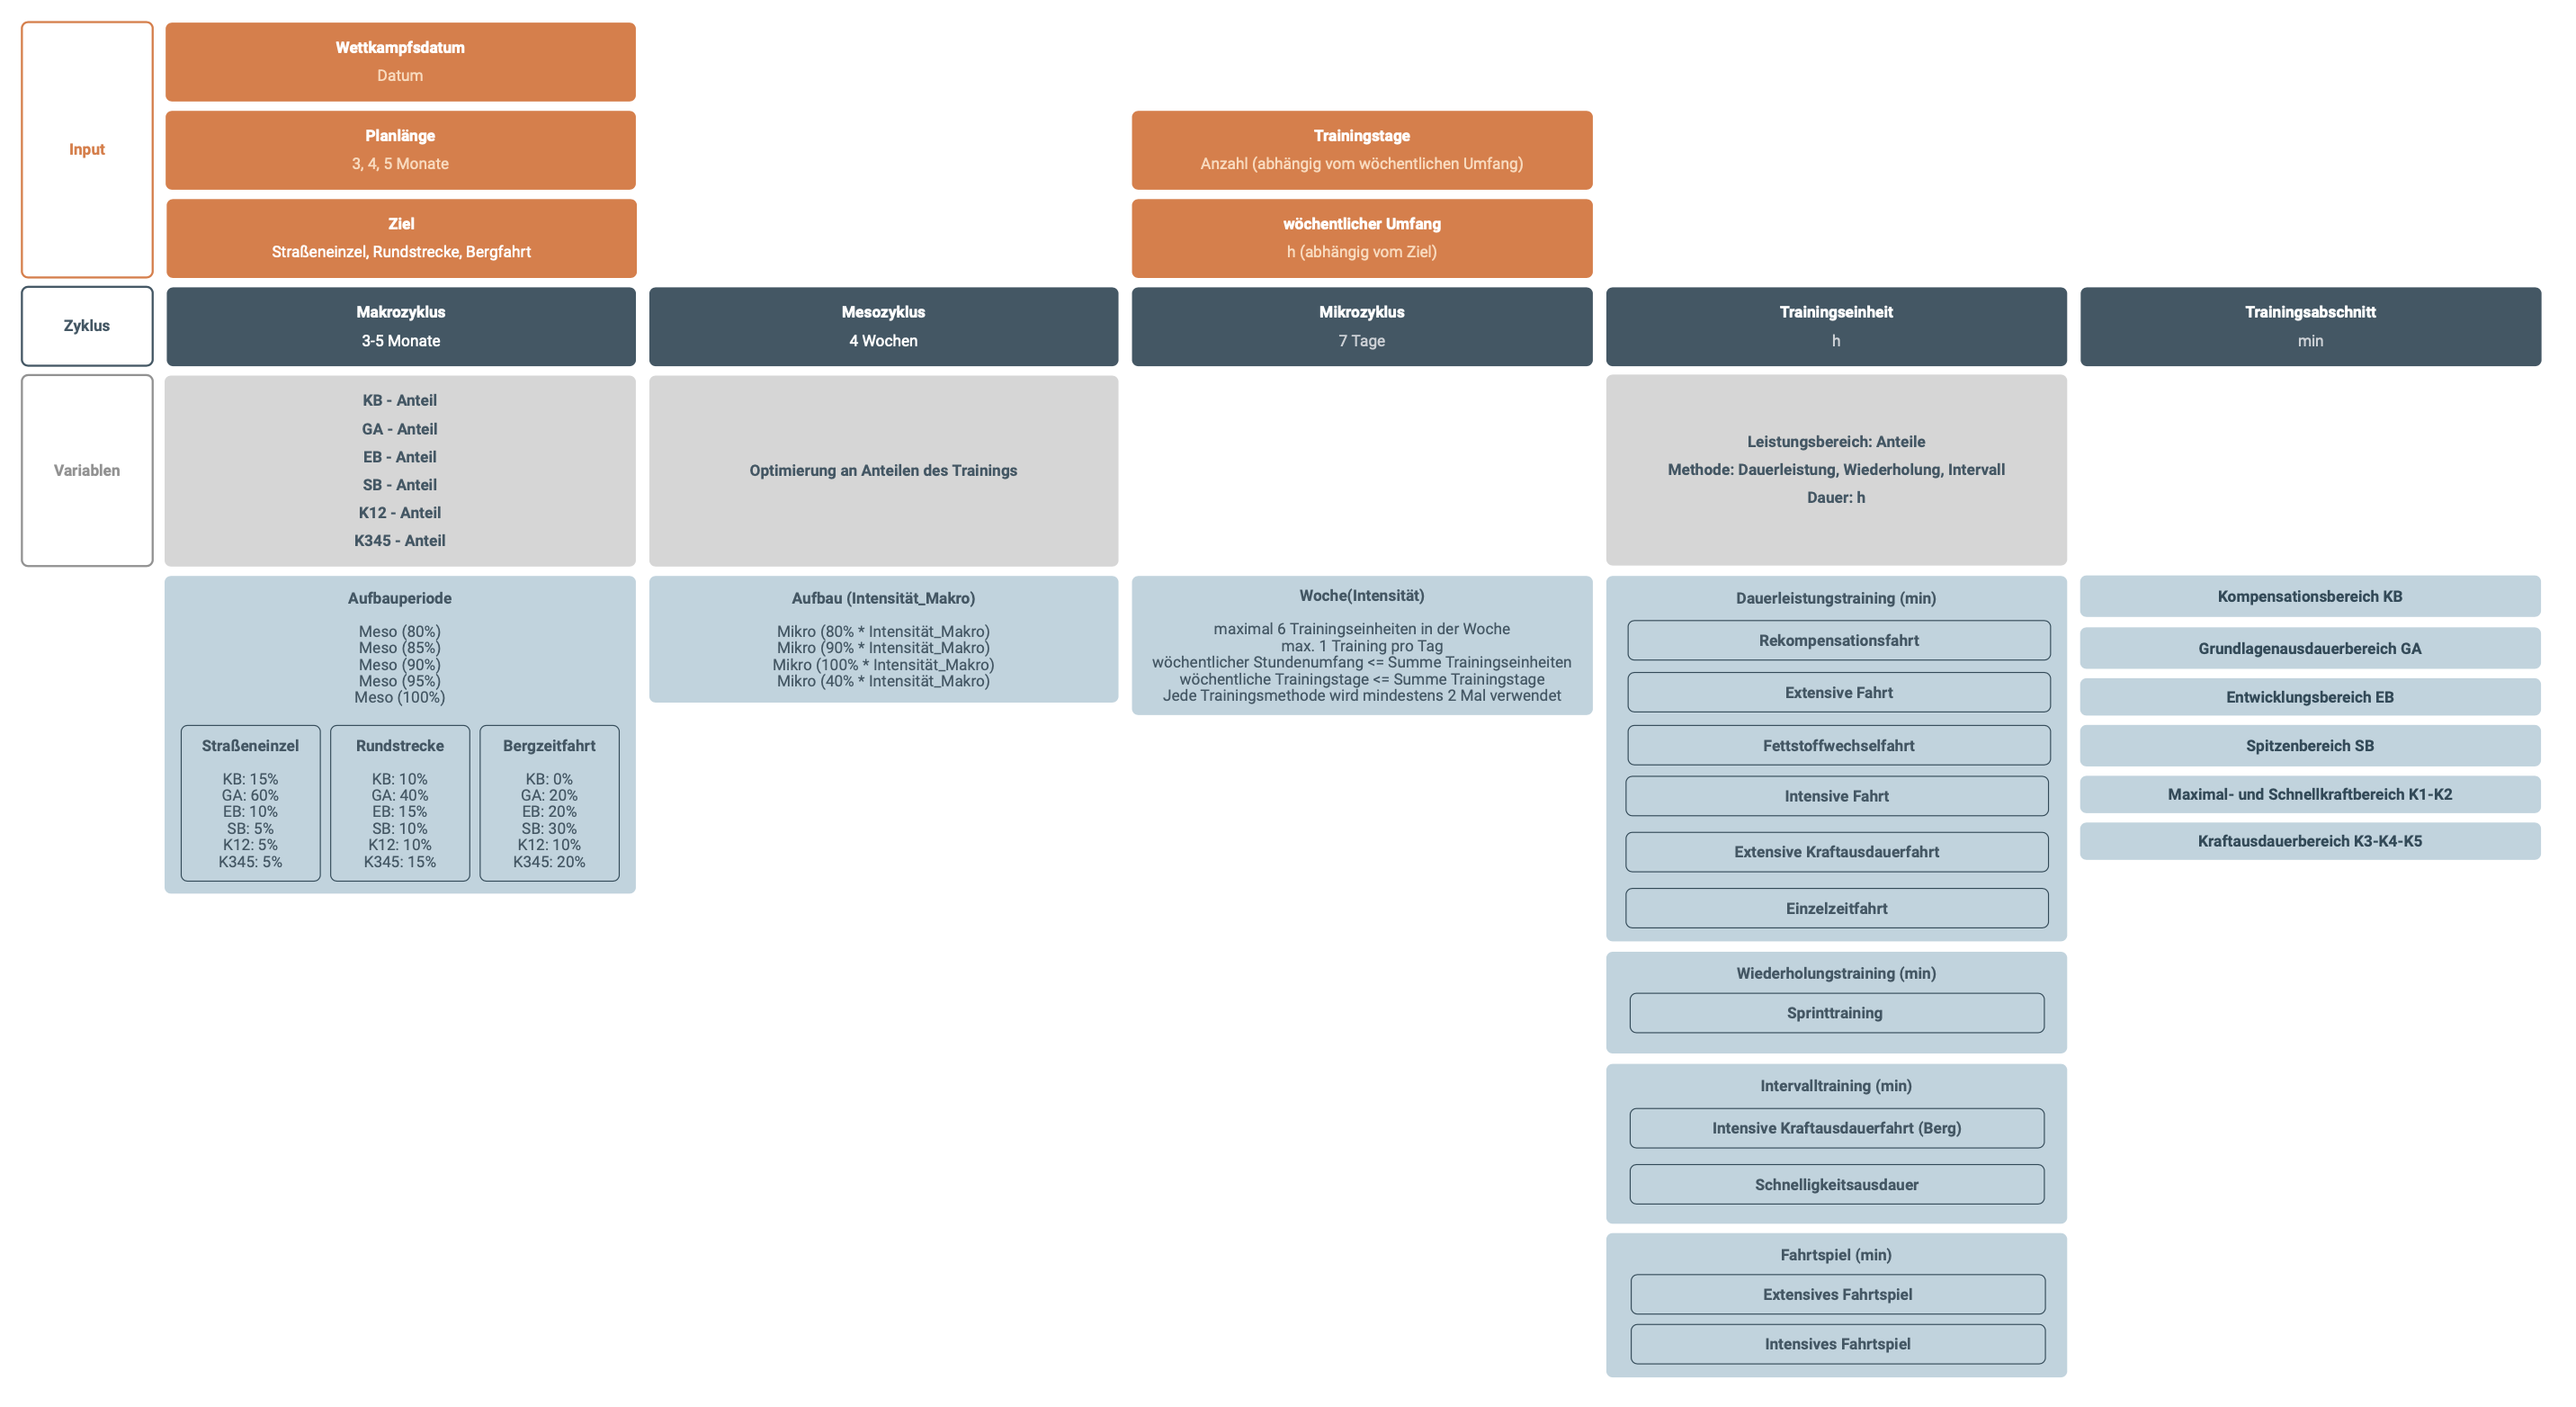
\includegraphics[height=\textwidth]{gfx/modellierung.png}
    \caption{Schema der Modellierung}
    \label{anhang:modellierung}
\end{figure}

\section{Trainingsplan im Freizeitsport}
\label{anhang:freizeitsport}

\section{Trainingsplan im Amateursport}
\label{anhang:amateursport}

\section{vollständige Modellierung}
\label{anhang:code:modell}

\begin{equation}
    \forall i \in [1, 28], min_i \mod 15 = 0
\end{equation} 
\begin{equation}
\begin{array}{c}
    \forall i \in [1, 28], kb_i \mod 5 = 0 \\
    \forall i \in [1, 28], ga_i \mod 5 = 0 \\
    \forall i \in [1, 28], eb_i \mod 5 = 0 \\
    \forall i \in [1, 28], sb_i \mod 5 = 0 \\
    \forall i \in [1, 28], k1_i \mod 5 = 0 \\
    \forall i \in [1, 28], k4_i \mod 5 = 0 \\
\end{array}
\end{equation}
\begin{equation} 
    \forall m \in ,|\{method_i = m | i \in [1, 28]\}| \geq 2
\end{equation} 
\begin{equation}
    \forall i = k * 7 + 1, k \in Z, \sum_{i}^{i+6} \text{duration}_i \leq max_{hours} 
\end{equation}
\begin{equation}
    \forall i \in \{ i = k * 7 + 1, k \in Z \}, \sum_{i}^{i+6} \text{duration}_i \leq max_{hours}
\end{equation}
\begin{equation}
    \forall i = k * 7 + 1, k \in Z, \sum_{i}^{i+6} \text{day}_i \leq max_{days}
\end{equation}
\begin{equation}
    method_i = \text{PAUSE} \Leftrightarrow minutes_i = 0
\end{equation}
\begin{equation}
    (method_i = \text{Dauerleistung})\Rightarrow t_i = \begin{array}{c}
            ([\![30, 120]\!], 0, 0, 0, 0, 0) \\ 
            \vee (0, [\![60, 240]\!], 0, 0, 0, 0) \\  
            \vee (0, [\![180, 360]\!], 0, 0, 0, 0) \\  
            \vee (0, 60, [\![15, 60]\!], 0, 0, 0) \\  
            \vee (0, [\![30, 60]\!], 0, 0, [\![30, 150]\!], 0) \\    
            \vee (0, 60, 0, [\![30, 60]\!], 0, 0) \\  
    \end{array}
\end{equation}
\begin{equation}
    (method_i = \text{Fahrtspiel})\Rightarrow t_i = \begin{array}{c}
            (0, [\![60, 240]\!], [\![60, 240]\!], 0, 0, 0) \\ 
        \vee (0, [\![60,180]\!], [\![60, 180]\!], [\![60, 180]\!], 0, 0)
    \end{array}
\end{equation}
\begin{equation}
    (method_i = \text{Intervall})\Rightarrow t_i = \begin{array}{c}
            (0, [\![30, 90]\!], 0, 0, 0, [\![15, 120]\!]) \\ 
        \vee (0, [\![60,180]\!], 0, [\![15, 45]\!], 0, 0)
    \end{array}
\end{equation}
\begin{equation}
    (method_i = \text{Wiederholung})\Rightarrow t_i = \begin{array}{c}
            (0, [\![30, 60]\!], 0, [\![15, 45]\!], 0, 0)
    \end{array}
\end{equation}
\begin{equation}
    \text{minimize} \sum_{m\in M} |\text{target}_m - \text{sum}_m|
\end{equation} 
